\section{Short bodies}

\begin{figure}
  \centering
  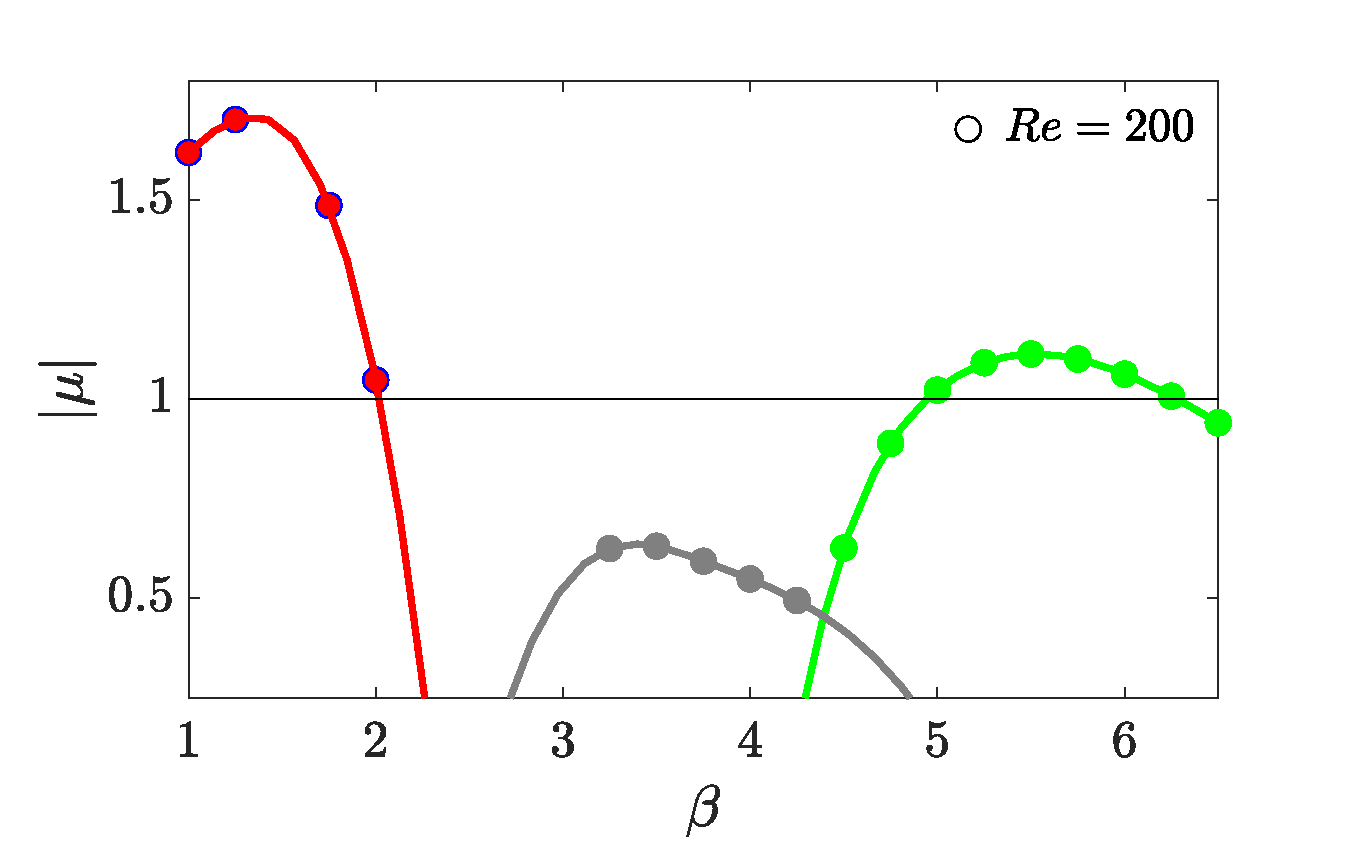
\includegraphics[width=0.49\textwidth]{./fig/AR1s/multipliers_AR1.eps}
  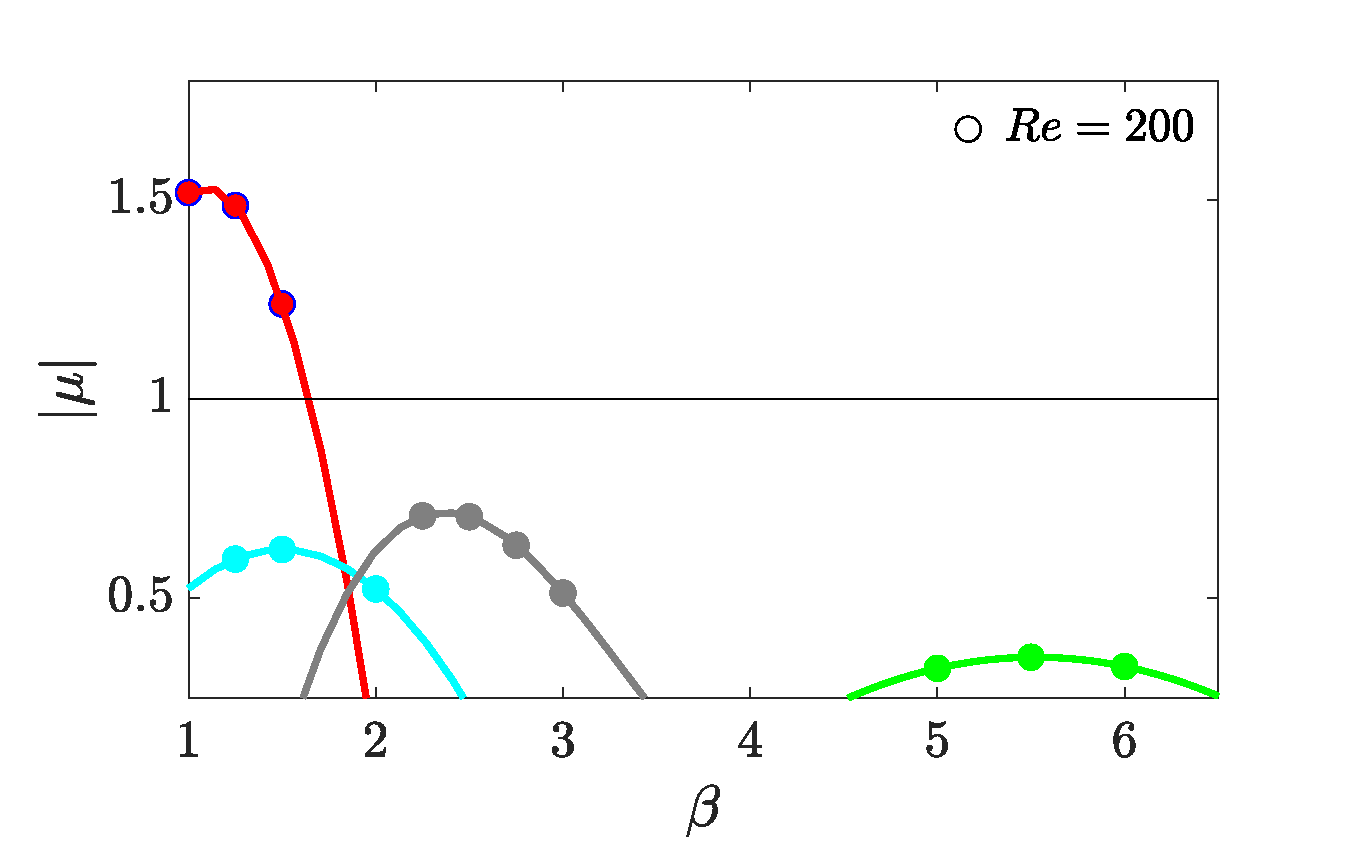
\includegraphics[width=0.49\textwidth]{./fig/AR1s/multipliers_AR1p25.eps}
  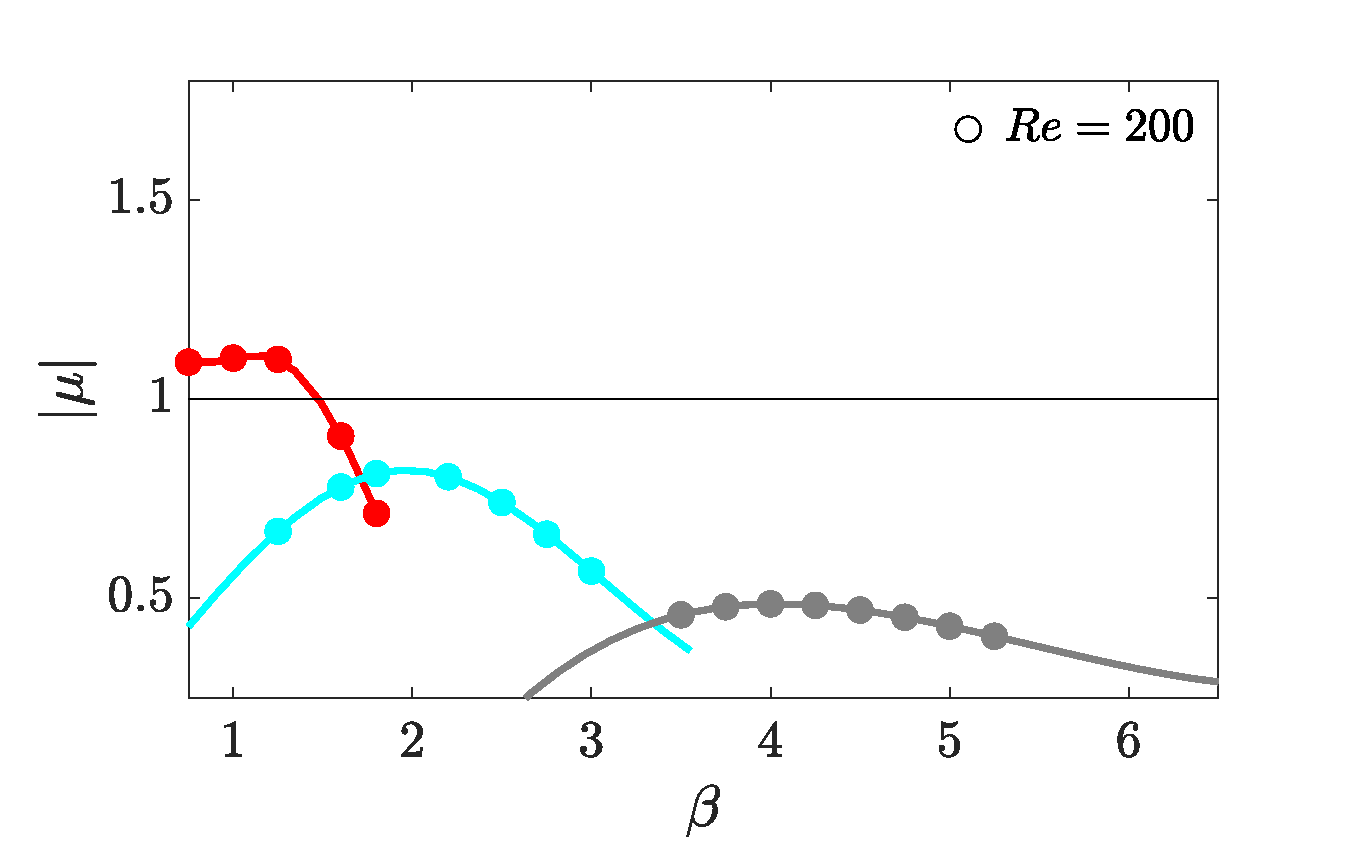
\includegraphics[width=0.49\textwidth]{./fig/AR1s/multipliers_AR1p5.eps}
  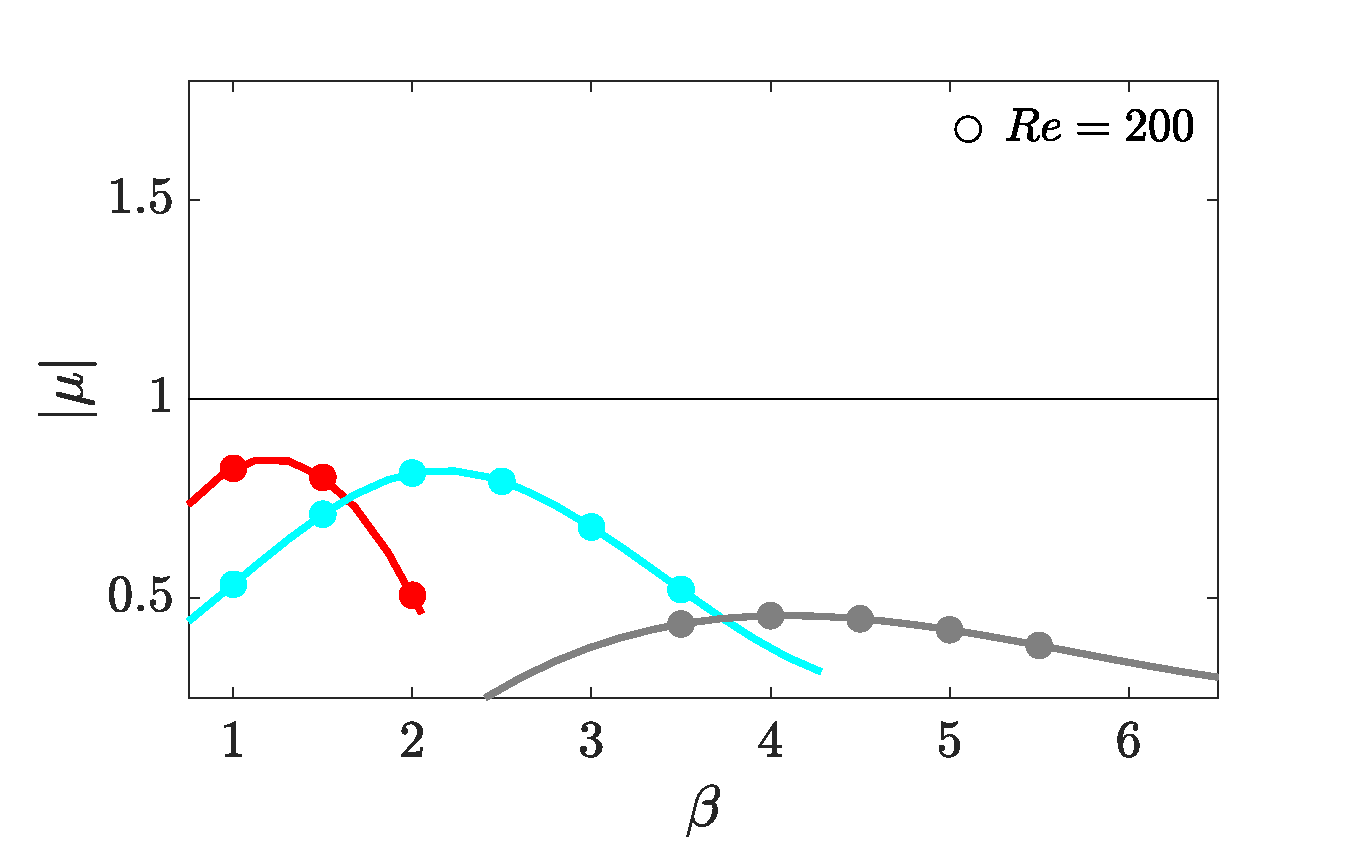
\includegraphics[width=0.49\textwidth]{./fig/AR1s/multipliers_AR1p75.eps} \\
  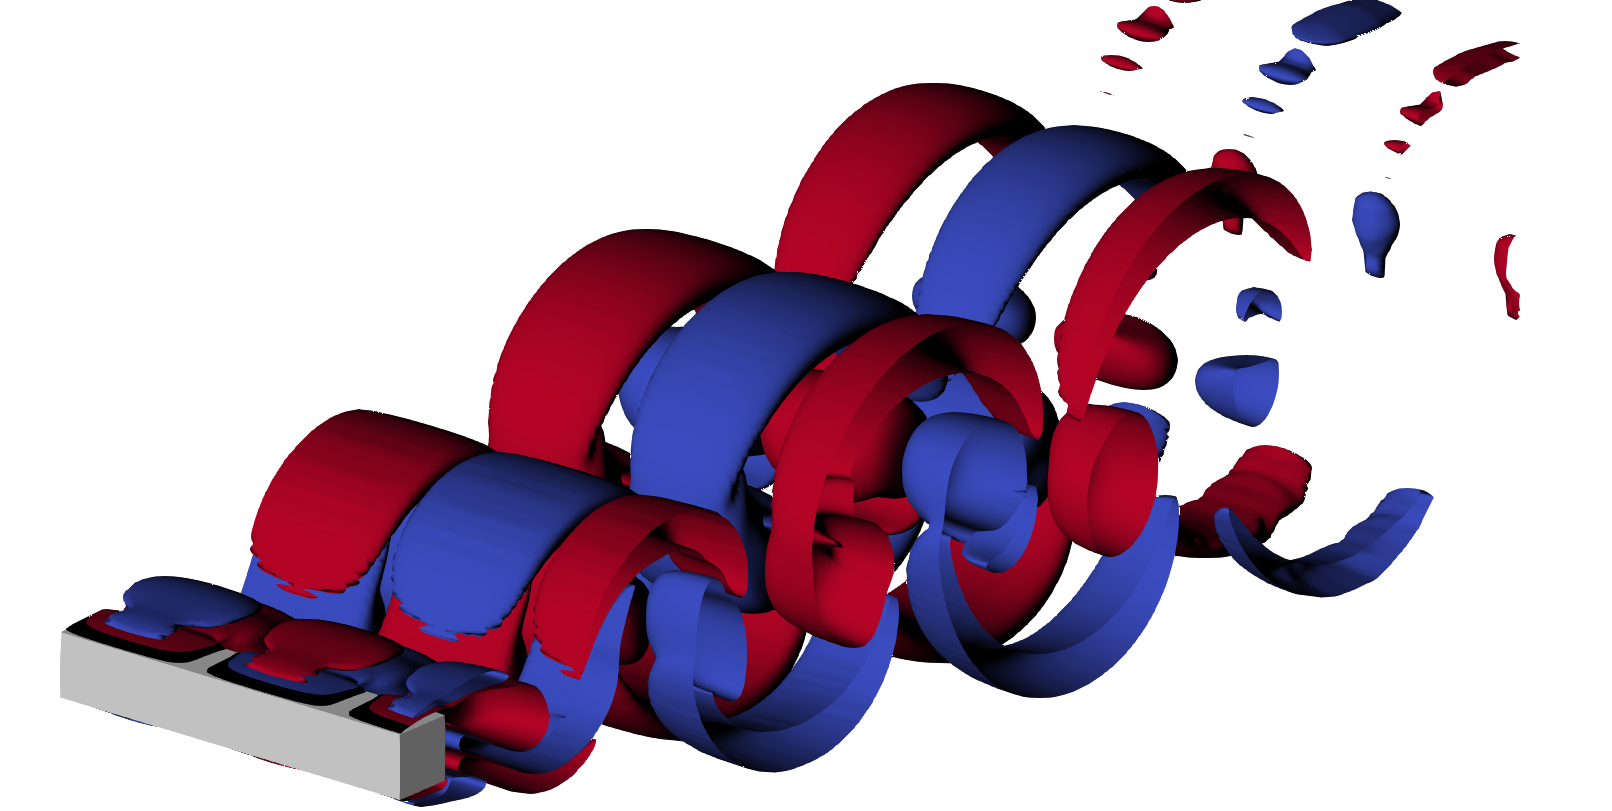
\includegraphics[width=0.32\textwidth]{./fig/AR1s/Floqetmode_beta_1p2_Re200_AR1_A.png}
  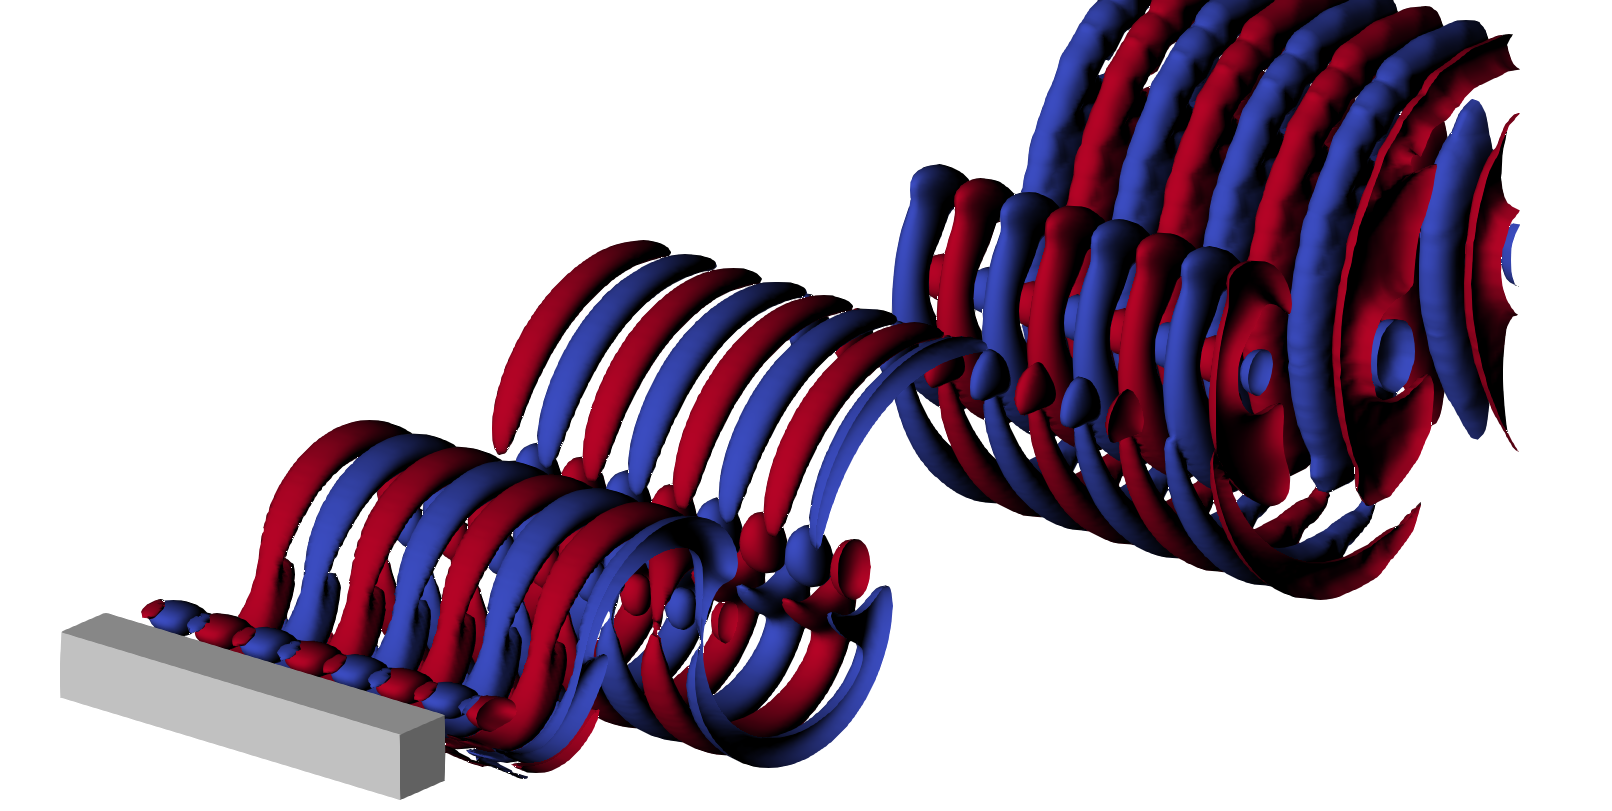
\includegraphics[width=0.32\textwidth]{./fig/AR1s/Floqetmode_beta_3p75_Re200_AR1_C.png}      
  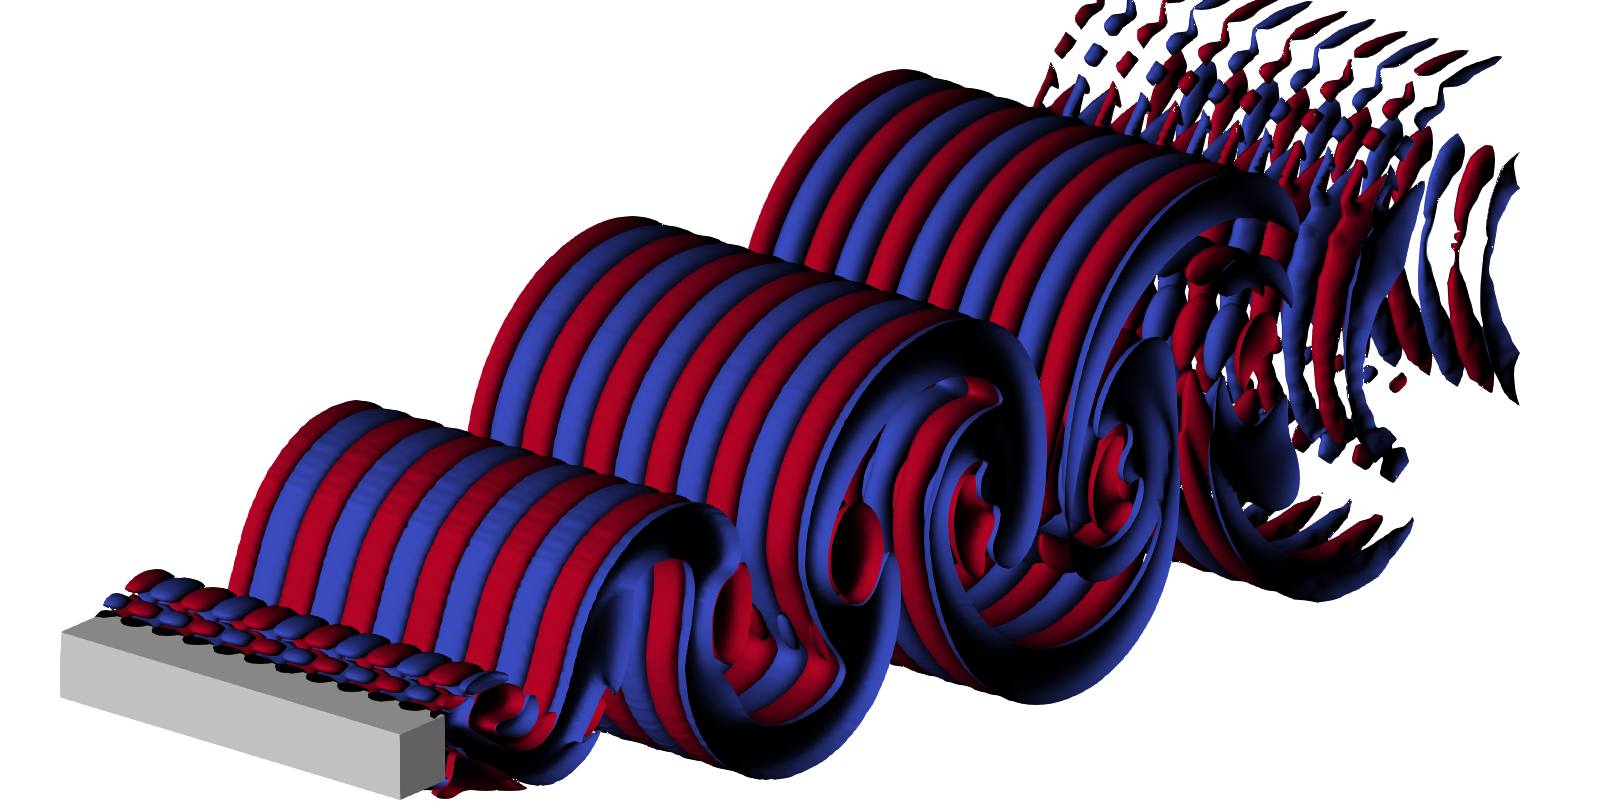
\includegraphics[width=0.32\textwidth]{./fig/AR1s/Floqetmode_beta_5p5_Re200_AR1_B.png}
  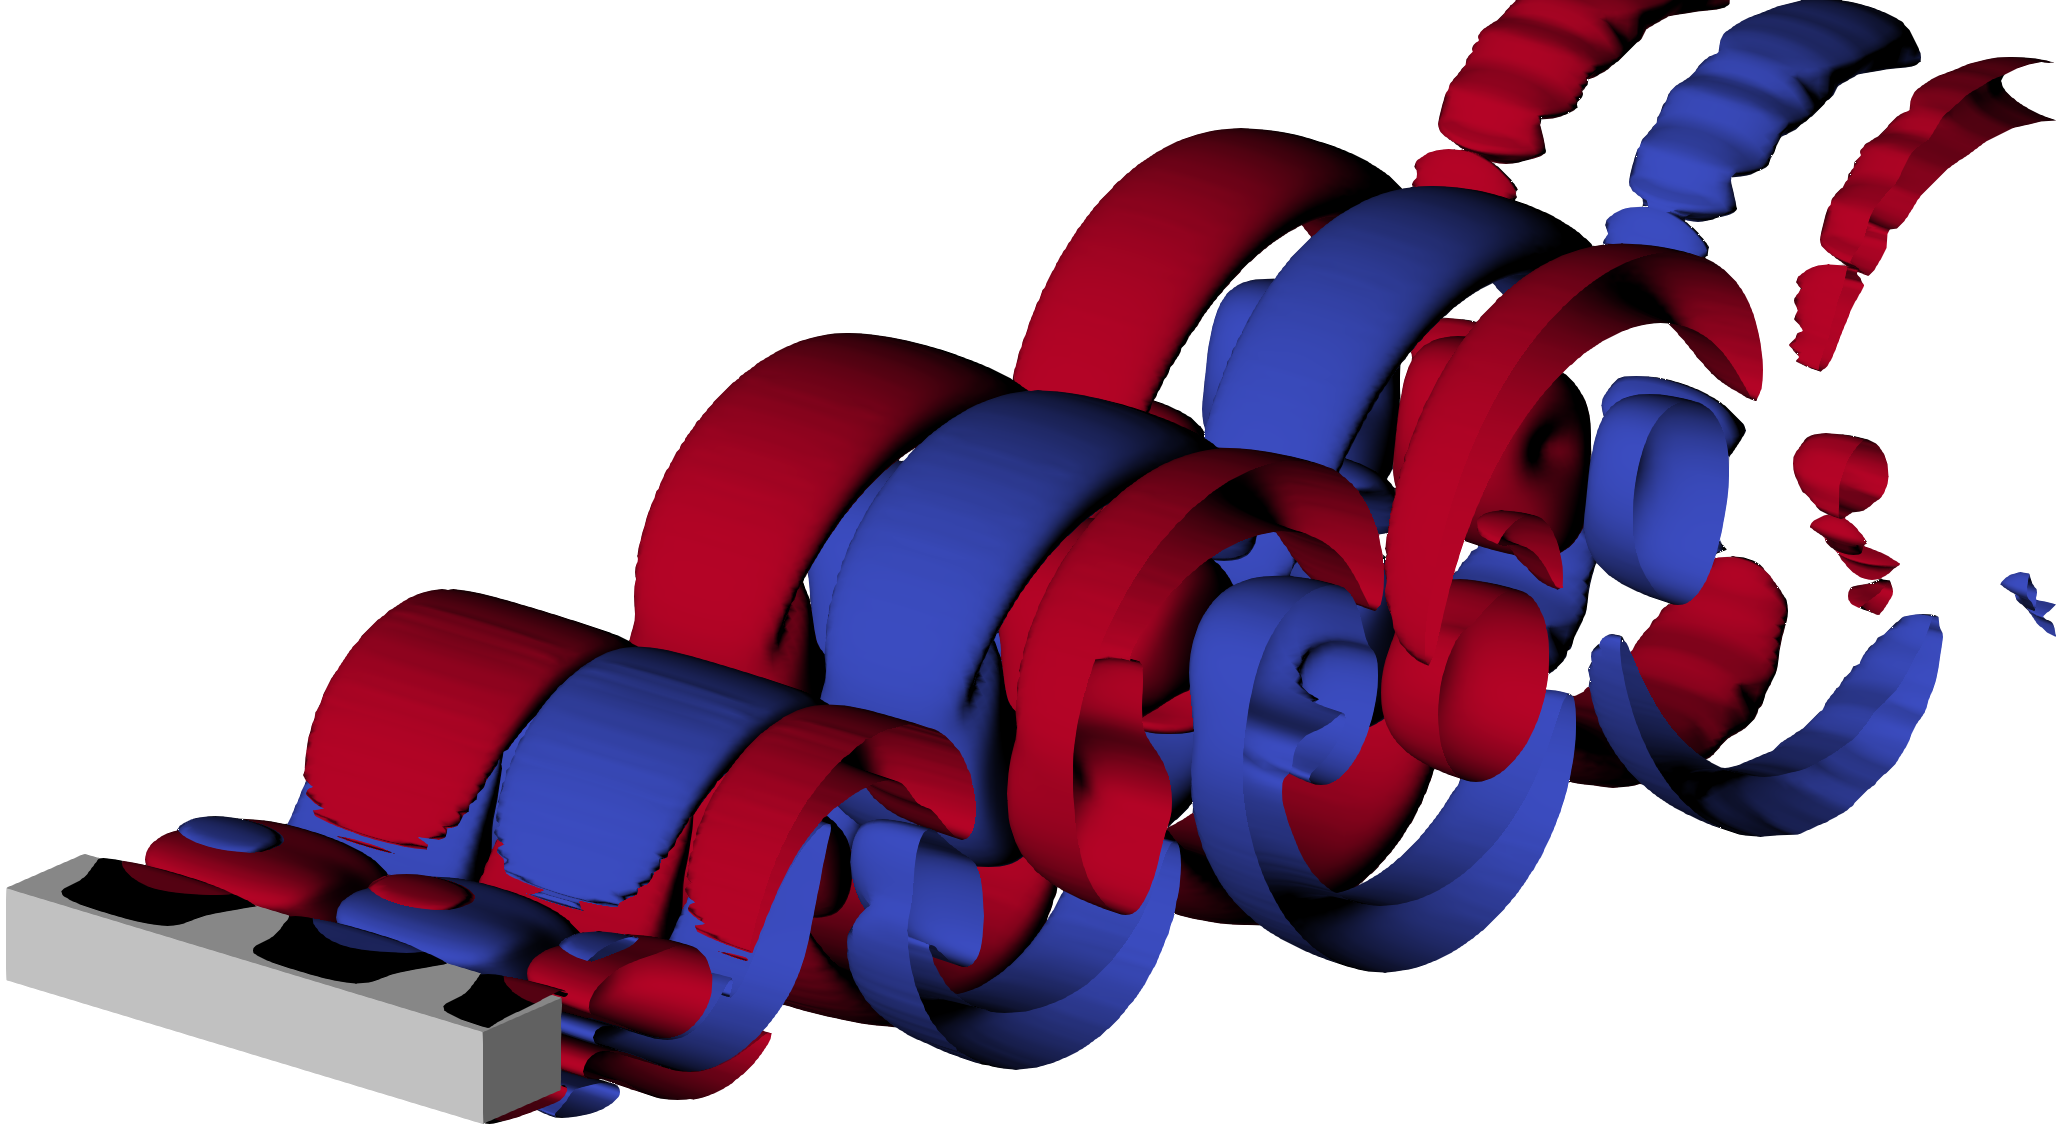
\includegraphics[width=0.32\textwidth]{./fig/AR1s/Floqetmode_beta_1p25_Re200_AR1p25_A.png}
  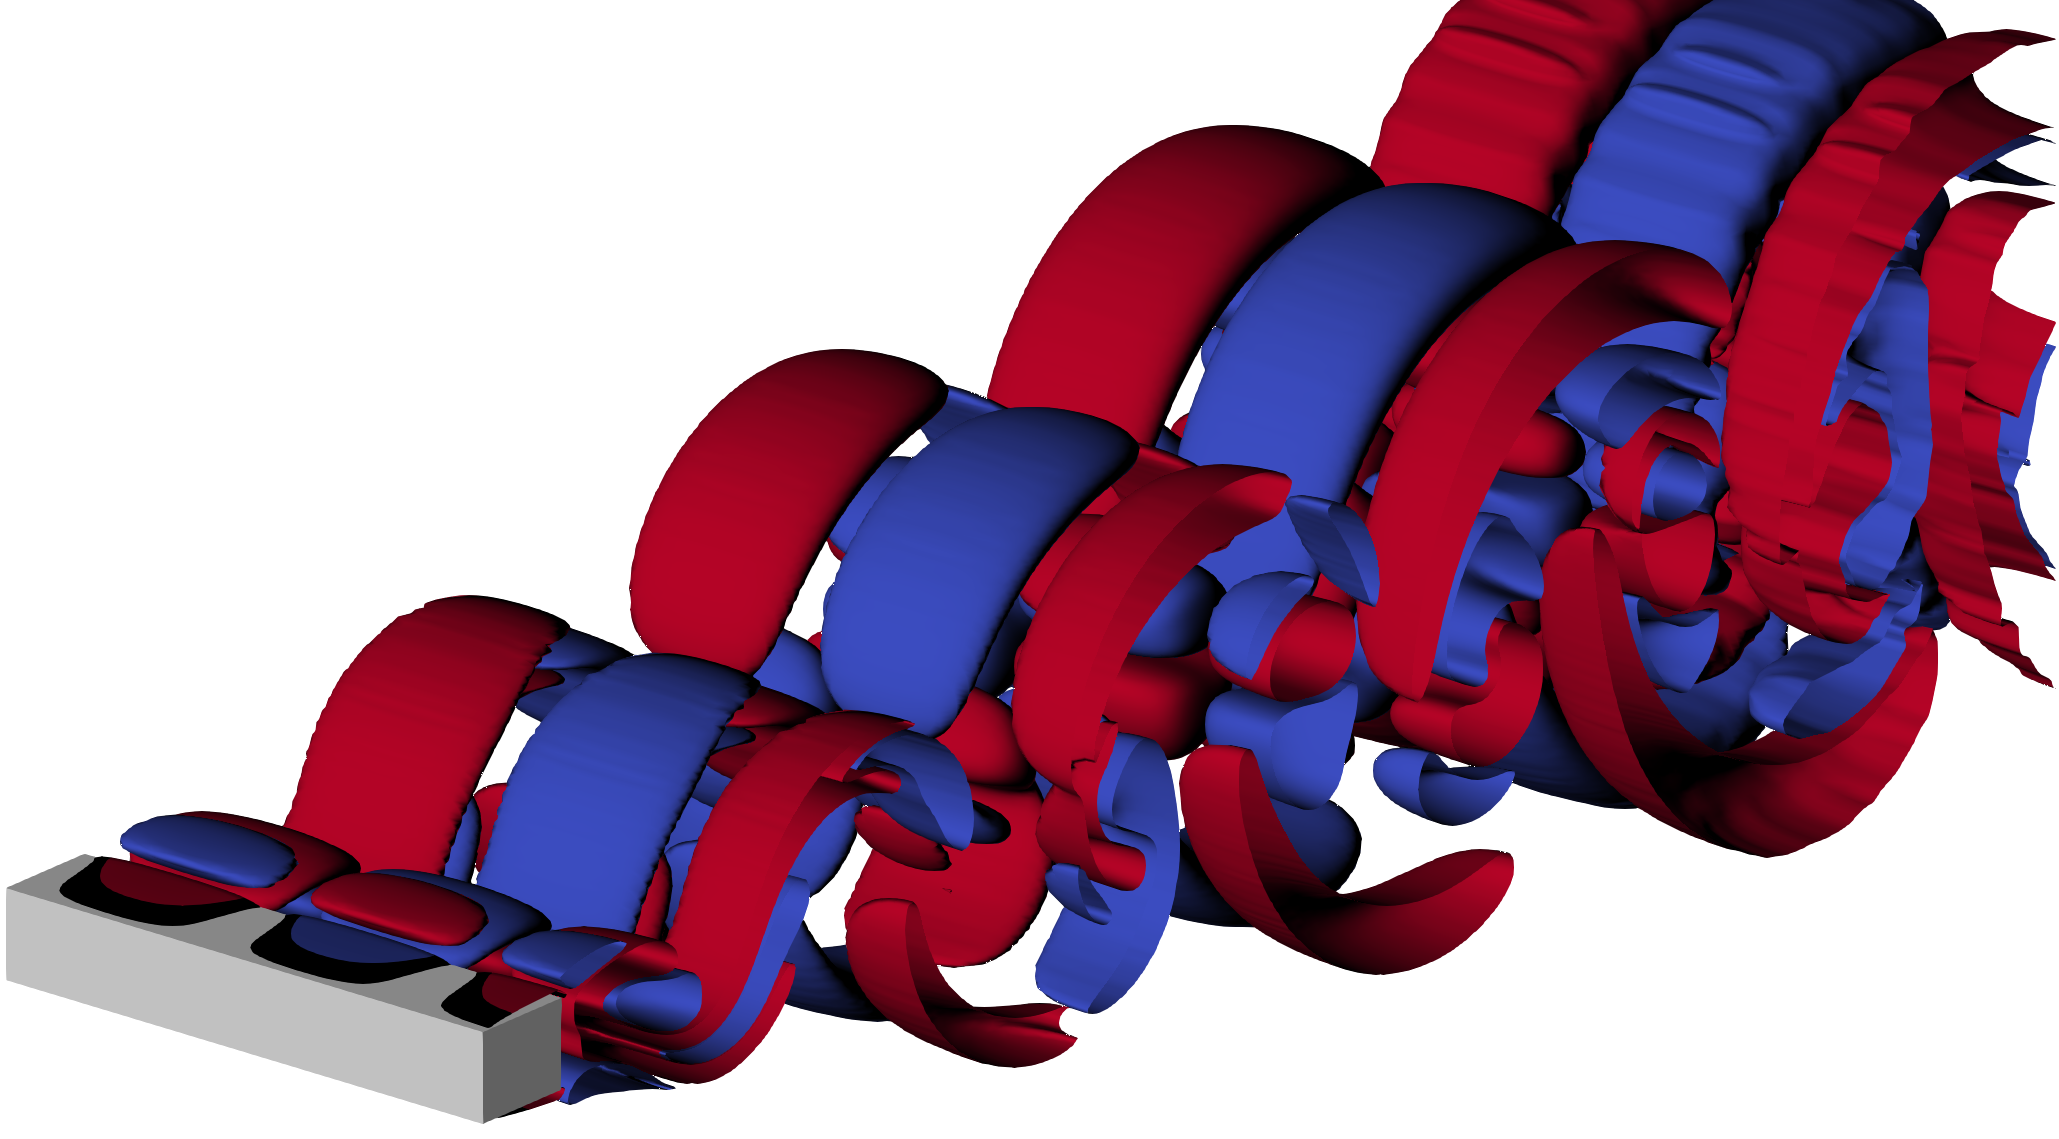
\includegraphics[width=0.32\textwidth]{./fig/AR1s/Floqetmode_beta_1p25_Re200_AR1p25_Bp.png}
  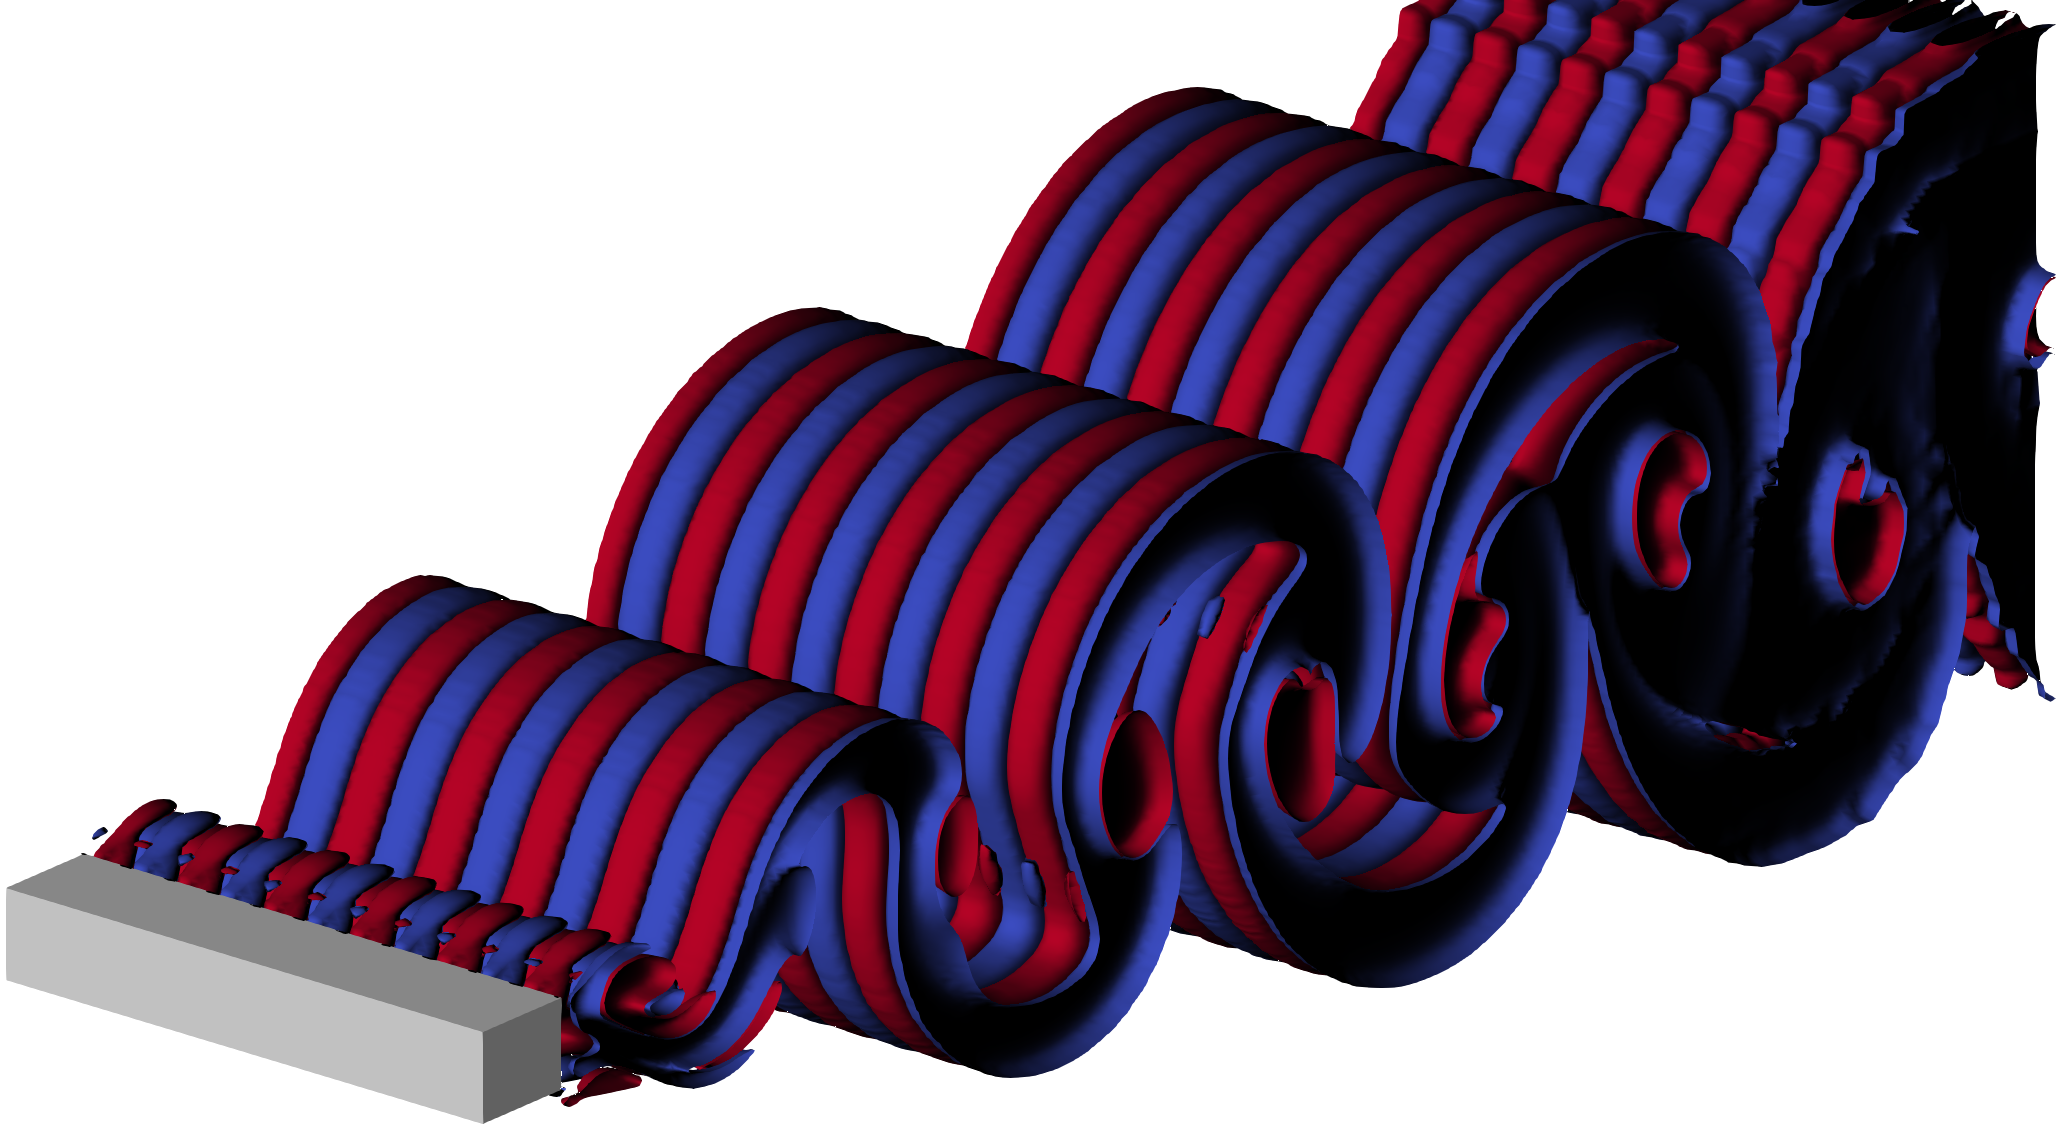
\includegraphics[width=0.32\textwidth]{./fig/AR1s/Floqetmode_beta_5p5_Re200_AR1p25_B.png}
  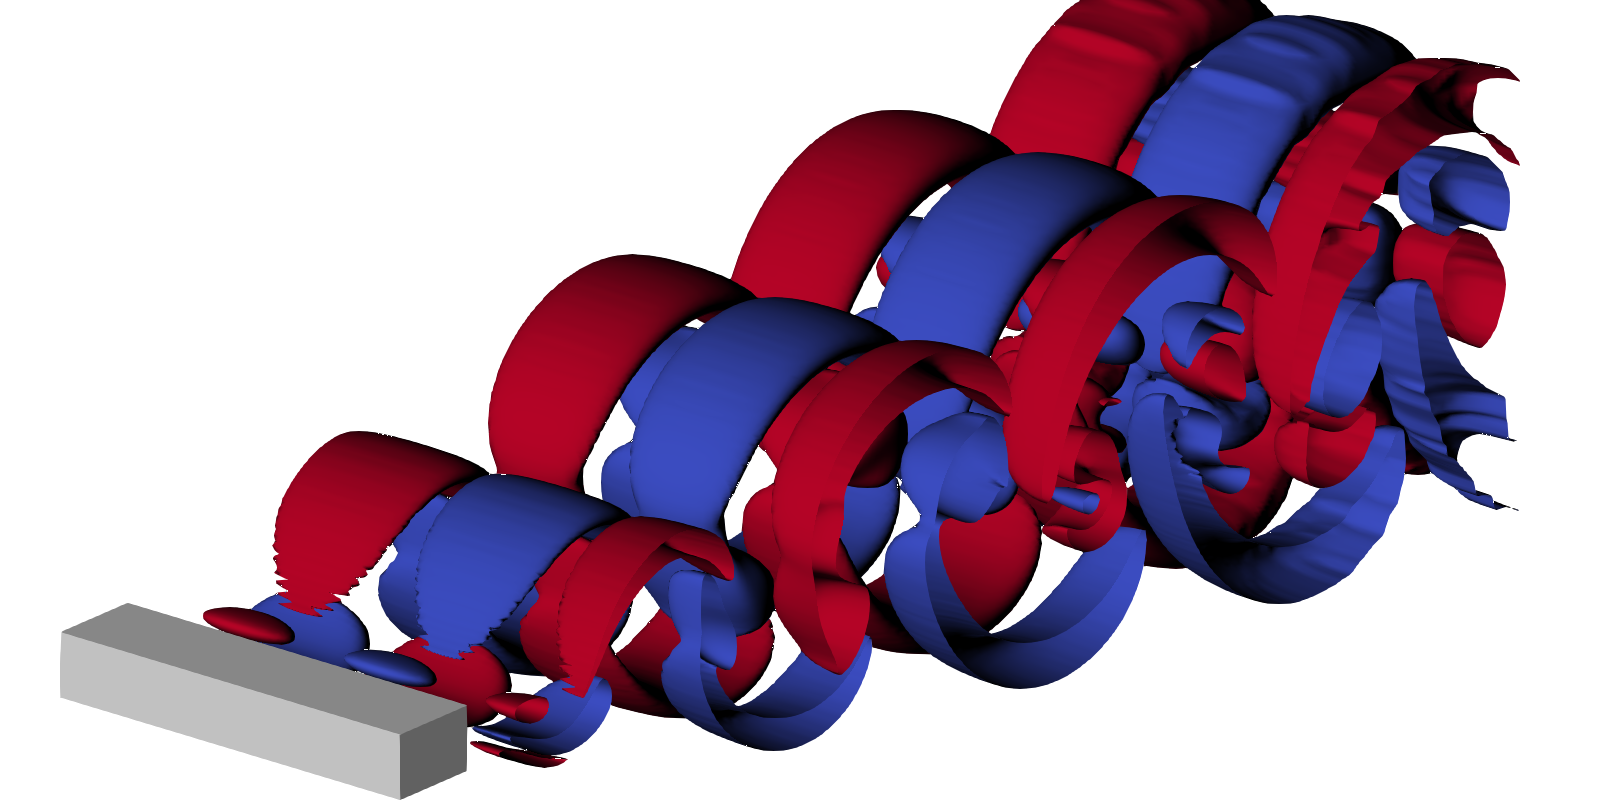
\includegraphics[width=0.32\textwidth]{./fig/AR1s/Floqetmode_beta_1p8_Re200_AR1p5_A.png}
  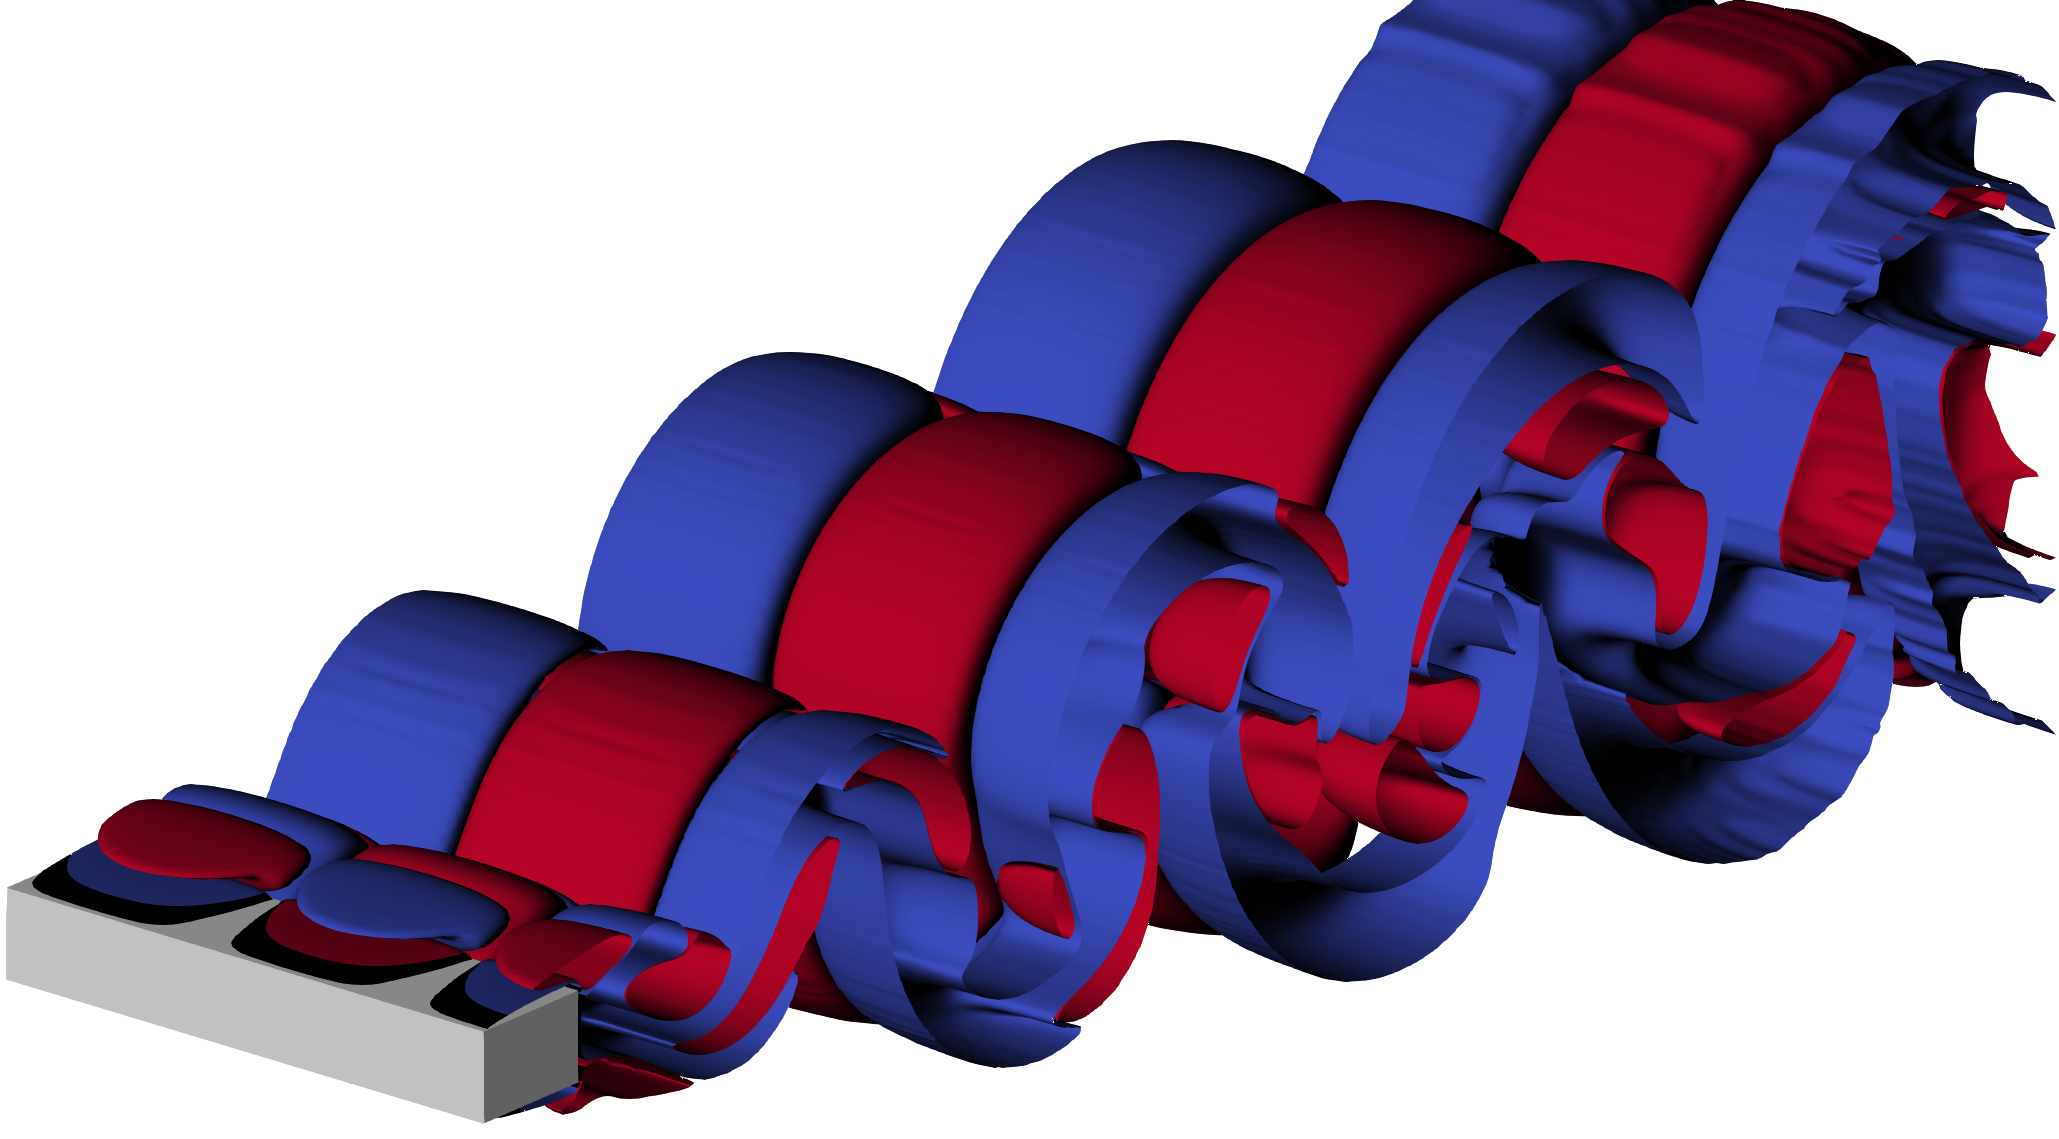
\includegraphics[width=0.32\textwidth]{./fig/AR1s/Floqetmode_beta_1p8_Re200_AR1p5_Bp.png}
  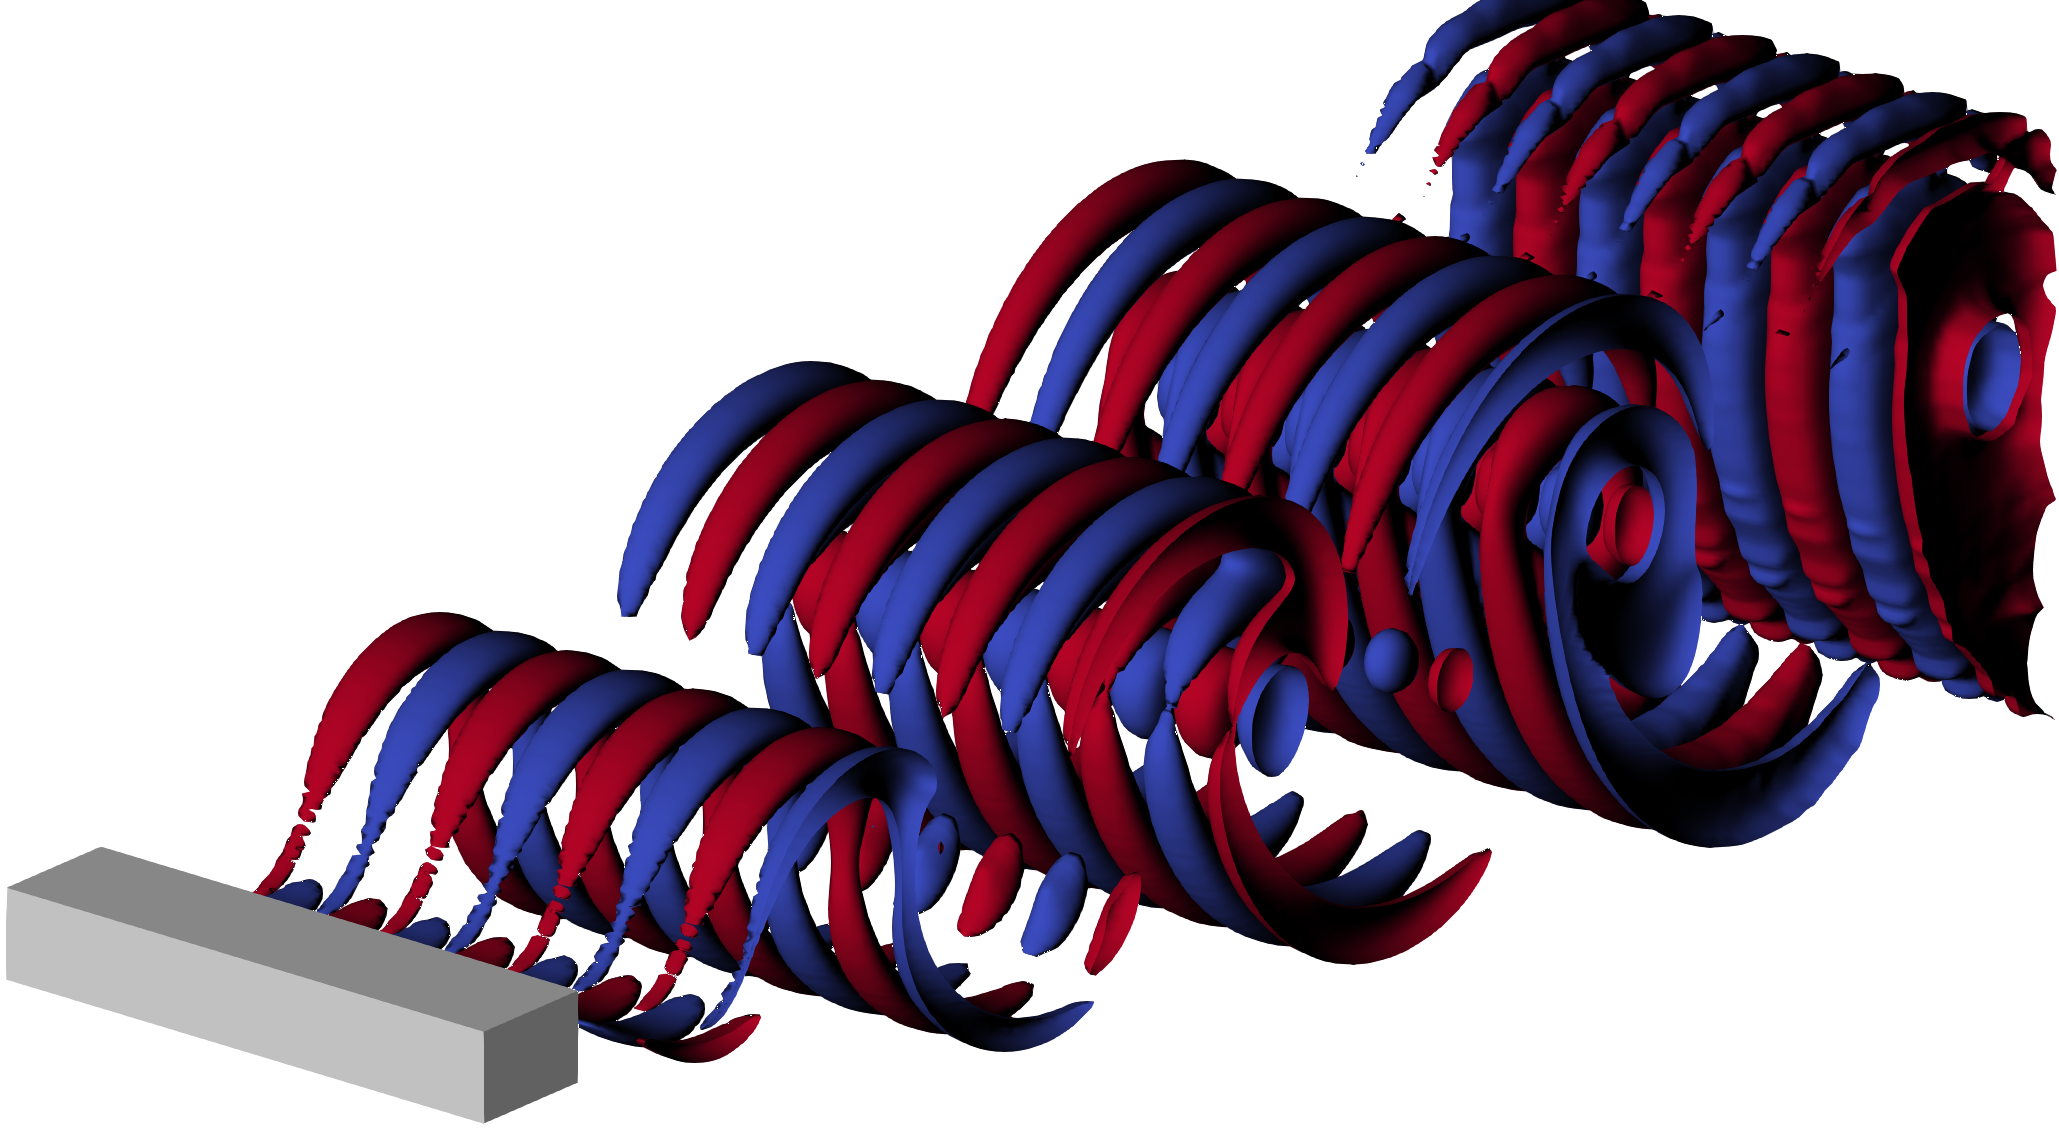
\includegraphics[width=0.32\textwidth]{./fig/AR1s/Floqetmode_beta_3p75_Re200_AR1p5_C.png}
  \caption{Top: multipliers for $\AR=1$, $\AR=1.25$ and $\AR=1.5$ at $Re=200$; the red line refers to mode $A$, the grey line to mode $C$, the green line to mode $B$ and the light blue line refers to mode $B'$. Mode $B'$ has the same spatio-temporal symmetry of mode $B$, but its characteristic wavelength is much smaller, being similar to that of mode $A$. This mode resembles that found for elongated bodies with elliptic leading edge by \cite{ryan-etal-2005}. The bottom panels show the Floquet modes associated with the different branches for the three $\AR$s. Top: Floquet modes for $\AR=1$ and $Re=200$, associated with mode A (left, $\beta=1.2$), mode C (centre, $\beta=3.75$) and mode $B$ (right, $\beta=5.5$). Centre: Floquet modes for $\AR=1.25$ and $Re=200$ associated with mode A (left, $\beta=1.25$), mode $B'$ (centre, $\beta = 1.25$) and mode $B$ (right, $\beta=5.5$). Bottom: Floquet modes for $\AR=1.5$ and $Re=200$ associated with mode A (left, $\beta=1.8$), mode $B'$ (centre, $\beta=1.8$) and mode $C$ (right, $\beta=3.75$). These are 3D reconstructions of the Floquet modes and the red/blue isosurfaces denote positive/negative streamwise vorticity.}
  \label{fig:xx}
\end{figure}

\begin{itemize}
  \item In this subsection we look at $\AR \in (1,2)$.
  \item Brifely recall the bifurcation scenario that has been observed for $\AR=1$, i.e. modes $A$, $QP$ and $B$.
  \item Give evidence of the influence of $\AR$ on these modes. They indeed stabilise a $\AR$ increases. Mode $B$ is not present any more for $\AR>1.25$. A new mode arises.
  \item Look at the symmetries of the modes.  
  \item \textcolor{blue}{For $\AR=1.25$ and $\AR=1.5$, modes $A$ and $B'$ become unstable is short succession. We can so use DNS to see what happens as $Re$ increases, and whether the flow changes from one mode to the other. (POD?)}
  \item Maybe we should add also $\AR=2$ and $\AR=2.5$ to see what happens.
\end{itemize}
